%%
%% Automatically generated file from DocOnce source
%% (https://github.com/hplgit/doconce/)
%%

% #define PREAMBLE

% #ifdef PREAMBLE
%-------------------- begin preamble ----------------------

\documentclass[%
oneside,                 % oneside: electronic viewing, twoside: printing
final,                   % draft: marks overfull hboxes, figures with paths
10pt]{article}

\listfiles               %  print all files needed to compile this document

\usepackage{relsize,makeidx,color,setspace,amsmath,amsfonts,amssymb}
\usepackage[table]{xcolor}
\usepackage{bm,ltablex,microtype}

\usepackage[pdftex]{graphicx}
\usepackage{fancyvrb}

\usepackage[T1]{fontenc}
%\usepackage[latin1]{inputenc}
\usepackage{ucs}
\usepackage[utf8x]{inputenc}

\usepackage{lmodern}         % Latin Modern fonts derived from Computer Modern

% Hyperlinks in PDF:
\definecolor{linkcolor}{rgb}{0,0,0.4}
\usepackage{hyperref}
\hypersetup{
    breaklinks=true,
    colorlinks=true,
    linkcolor=linkcolor,
    urlcolor=linkcolor,
    citecolor=black,
    filecolor=black,
    %filecolor=blue,
    pdfmenubar=true,
    pdftoolbar=true,
    bookmarksdepth=3   % Uncomment (and tweak) for PDF bookmarks with more levels than the TOC
    }
%\hyperbaseurl{}   % hyperlinks are relative to this root

\setcounter{tocdepth}{2}  % levels in table of contents

% Tricks for having figures close to where they are defined:
% 1. define less restrictive rules for where to put figures
\setcounter{topnumber}{2}
\setcounter{bottomnumber}{2}
\setcounter{totalnumber}{4}
\renewcommand{\topfraction}{0.95}
\renewcommand{\bottomfraction}{0.95}
\renewcommand{\textfraction}{0}
\renewcommand{\floatpagefraction}{0.75}
% floatpagefraction must always be less than topfraction!
% 2. ensure all figures are flushed before next section
\usepackage[section]{placeins}
% 3. enable begin{figure}[H] (often leads to ugly pagebreaks)
%\usepackage{float}\restylefloat{figure}

% --- fancyhdr package for fancy headers ---
\usepackage{fancyhdr}
\fancyhf{} % sets both header and footer to nothing
\renewcommand{\headrulewidth}{0pt}
\fancyfoot[LE,RO]{\thepage}
% Ensure copyright on titlepage (article style) and chapter pages (book style)
\fancypagestyle{plain}{
  \fancyhf{}
  \fancyfoot[C]{{\footnotesize \copyright\ 2018-2020, Christian Forssén. Released under CC Attribution-NonCommercial 4.0 license}}
%  \renewcommand{\footrulewidth}{0mm}
  \renewcommand{\headrulewidth}{0mm}
}
% Ensure copyright on titlepages with \thispagestyle{empty}
\fancypagestyle{empty}{
  \fancyhf{}
  \fancyfoot[C]{{\footnotesize \copyright\ 2018-2020, Christian Forssén. Released under CC Attribution-NonCommercial 4.0 license}}
  \renewcommand{\footrulewidth}{0mm}
  \renewcommand{\headrulewidth}{0mm}
}

\pagestyle{fancy}


\usepackage[framemethod=TikZ]{mdframed}

% --- begin definitions of admonition environments ---

% Admonition style "mdfbox" is an oval colored box based on mdframed
% "notice" admon
\definecolor{mdfbox_notice_background}{rgb}{1,1,1}
\newmdenv[
  skipabove=15pt,
  skipbelow=15pt,
  outerlinewidth=0,
  backgroundcolor=mdfbox_notice_background,
  linecolor=black,
  linewidth=2pt,       % frame thickness
  frametitlebackgroundcolor=mdfbox_notice_background,
  frametitlerule=true,
  frametitlefont=\normalfont\bfseries,
  shadow=false,        % frame shadow?
  shadowsize=11pt,
  leftmargin=0,
  rightmargin=0,
  roundcorner=5,
  needspace=0pt,
]{notice_mdfboxmdframed}

\newenvironment{notice_mdfboxadmon}[1][]{
\begin{notice_mdfboxmdframed}[frametitle=#1]
}
{
\end{notice_mdfboxmdframed}
}

% Admonition style "mdfbox" is an oval colored box based on mdframed
% "summary" admon
\definecolor{mdfbox_summary_background}{rgb}{1,1,1}
\newmdenv[
  skipabove=15pt,
  skipbelow=15pt,
  outerlinewidth=0,
  backgroundcolor=mdfbox_summary_background,
  linecolor=black,
  linewidth=2pt,       % frame thickness
  frametitlebackgroundcolor=mdfbox_summary_background,
  frametitlerule=true,
  frametitlefont=\normalfont\bfseries,
  shadow=false,        % frame shadow?
  shadowsize=11pt,
  leftmargin=0,
  rightmargin=0,
  roundcorner=5,
  needspace=0pt,
]{summary_mdfboxmdframed}

\newenvironment{summary_mdfboxadmon}[1][]{
\begin{summary_mdfboxmdframed}[frametitle=#1]
}
{
\end{summary_mdfboxmdframed}
}

% Admonition style "mdfbox" is an oval colored box based on mdframed
% "warning" admon
\definecolor{mdfbox_warning_background}{rgb}{1,1,1}
\newmdenv[
  skipabove=15pt,
  skipbelow=15pt,
  outerlinewidth=0,
  backgroundcolor=mdfbox_warning_background,
  linecolor=black,
  linewidth=2pt,       % frame thickness
  frametitlebackgroundcolor=mdfbox_warning_background,
  frametitlerule=true,
  frametitlefont=\normalfont\bfseries,
  shadow=false,        % frame shadow?
  shadowsize=11pt,
  leftmargin=0,
  rightmargin=0,
  roundcorner=5,
  needspace=0pt,
]{warning_mdfboxmdframed}

\newenvironment{warning_mdfboxadmon}[1][]{
\begin{warning_mdfboxmdframed}[frametitle=#1]
}
{
\end{warning_mdfboxmdframed}
}

% Admonition style "mdfbox" is an oval colored box based on mdframed
% "question" admon
\definecolor{mdfbox_question_background}{rgb}{1,1,1}
\newmdenv[
  skipabove=15pt,
  skipbelow=15pt,
  outerlinewidth=0,
  backgroundcolor=mdfbox_question_background,
  linecolor=black,
  linewidth=2pt,       % frame thickness
  frametitlebackgroundcolor=mdfbox_question_background,
  frametitlerule=true,
  frametitlefont=\normalfont\bfseries,
  shadow=false,        % frame shadow?
  shadowsize=11pt,
  leftmargin=0,
  rightmargin=0,
  roundcorner=5,
  needspace=0pt,
]{question_mdfboxmdframed}

\newenvironment{question_mdfboxadmon}[1][]{
\begin{question_mdfboxmdframed}[frametitle=#1]
}
{
\end{question_mdfboxmdframed}
}

% Admonition style "mdfbox" is an oval colored box based on mdframed
% "block" admon
\definecolor{mdfbox_block_background}{rgb}{1,1,1}
\newmdenv[
  skipabove=15pt,
  skipbelow=15pt,
  outerlinewidth=0,
  backgroundcolor=mdfbox_block_background,
  linecolor=black,
  linewidth=2pt,       % frame thickness
  frametitlebackgroundcolor=mdfbox_block_background,
  frametitlerule=true,
  frametitlefont=\normalfont\bfseries,
  shadow=false,        % frame shadow?
  shadowsize=11pt,
  leftmargin=0,
  rightmargin=0,
  roundcorner=5,
  needspace=0pt,
]{block_mdfboxmdframed}

\newenvironment{block_mdfboxadmon}[1][]{
\begin{block_mdfboxmdframed}[frametitle=#1]
}
{
\end{block_mdfboxmdframed}
}

% --- end of definitions of admonition environments ---

% prevent orhpans and widows
\clubpenalty = 10000
\widowpenalty = 10000

% --- end of standard preamble for documents ---


\usepackage[swedish]{babel}

\raggedbottom
\makeindex
\usepackage[totoc]{idxlayout}   % for index in the toc
\usepackage[nottoc]{tocbibind}  % for references/bibliography in the toc

%-------------------- end preamble ----------------------

\begin{document}

% matching end for #ifdef PREAMBLE
% #endif

\newcommand{\exercisesection}[1]{\subsection*{#1}}

\input{newcommands_keep}

% ------------------- main content ----------------------



% ----------------- title -------------------------

\thispagestyle{empty}

\begin{center}
{\LARGE\bf
\begin{spacing}{1.25}
Learning from data: Model Validation and Regularization
\end{spacing}
}
\end{center}

% ----------------- author(s) -------------------------

\begin{center}
{\bf Christian Forssén}
\end{center}

    \begin{center}
% List of all institutions:
\centerline{{\small Department of Physics, Chalmers University of Technology, Sweden}}
\end{center}
    
% ----------------- end author(s) -------------------------

% --- begin date ---
\begin{center}
Sep 7, 2020
\end{center}
% --- end date ---

\vspace{1cm}


In this lecture we will continue to explore linear regression and we will encounter several concepts that are common for machine learning methods. These concepts are:
\begin{itemize}
  \item Model validation

  \item Overfitting and underfitting

  \item Bias-variance-tradeoff

  \item Regularization

  \item Model hyperparameters

  \item Gradient descent optimization

  \item Learning curves
\end{itemize}

\noindent
This lecture is accompanied by a demonstration Jupyter notebook. Furthermore, you will get your own experience with these concepts when working on the linear regression exercise and the problem set.

The lecture is based and inspired by material in several good textbooks: in particular chapter 4 in \href{{http://shop.oreilly.com/product/0636920052289.do}}{Hands‑On Machine Learning with Scikit‑Learn and TensorFlow} by Aurelien Geron and chapter 5 in the 
\href{{http://shop.oreilly.com/product/0636920034919.do}}{Python Data Science Handbook} by Jake VanderPlas.
The cross-validation example with Ridge Regularization is taken from teaching material developed by Morten Hjorth-Jensen at the Department of Physics, University of Oslo {\&} Department of Physics and Astronomy and National Superconducting Cyclotron Laboratory, Michigan State University. 

% !split
\section{Model validation}

% !split
\subsection{Over- and underfitting}

Overfitting and underfitting are common problems in data analysis and machine learning. Both extremes are illustrated in Fig.~\ref{fig-over_under_fitting} from the demonstration notebook.


\begin{figure}[!ht]  % fig-over_under_fitting
  \centerline{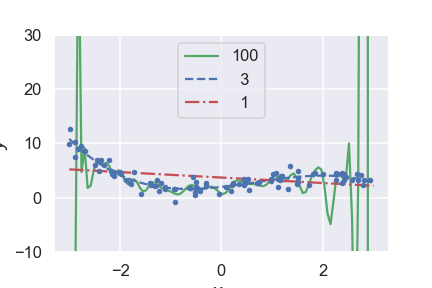
\includegraphics[width=0.8\linewidth]{fig/over_under_fitting.png}}
  \caption{
  The first-order polynomial model is clearly underfitting the data, while the very high degree model is overfitting it trying to reproduce variations that are clearly noise. \label{fig-over_under_fitting}
  }
\end{figure}
%\clearpage % flush figures fig-over_under_fitting


The following quote from an unknown source provides a concise definition of overfitting and underfitting:

\begin{quote}
A model overfits if it fits noise as much as data and underfits if it considers variability in data to be noise while it is actually not.
\end{quote}


The question is then: How do we detect these problems and how can we reduce them.

We can detect over- and underfitting by employing holdout sets, also known as \emph{validation} sets. This means that we only use a fraction of the data for training the model, and save the rest for validation purposes. I.e. we optimize the model parameters to best fit the training data, and then measure e.g.~the mean-square error (MSE) of the model predictions for the validation set. 

An underfit model has a \emph{high bias}, which means that it gives a rather poor fit and the performance metric will be rather bad (large error). This will be true for both the training and the validation sets.

An overfit model typically has a very \emph{large varianc}, i.e.~the model predictions reveal larger variance than the data itself. We will discuss this in more detail further down. High variance models typically perform much better on the training set than on the validation set. 

Alternatively, a telltale sign for overfitting is the appearance of very large fit parameters that are needed for the fine tunings of cancellations of different terms in the model. The fits from our example has the following root-mean-square parameters

\[
\theta_\mathrm{rms} \equiv \frac{1}{p} \sqrt{ \sum_{i=0}^p \theta_i^2 } \equiv \| \theta \|_2^2 / p.
\]



\begin{tabular}{rr}
\hline
\multicolumn{1}{r}{ order } & \multicolumn{1}{r}{ $\theta_\mathrm{rms}$ } \\
\hline
1     & 3.0e-01               \\
3     & 1.2e+00               \\
100   & 6.3e+12               \\
\hline
\end{tabular}


\noindent

% !split
\subsection{Regularization: Ridge and Lasso}

Assuming that overfitting is characterized by large fit parameters, we can attempt to avoid this scenario by \emph{regularizing} the model parameters. We will introduce two kinds of regularization: Ridge and Lasso. In addition, so called elastic net regularization is also in use and basically corresponds to a linear combination of the Ridge and Lasso penalty functions.

Let us remind ourselves about the expression for the standard Mean Squared Error (MSE) which we used to define our cost function and the equations for the ordinary least squares (OLS) method. That is our optimization problem is
\[
\bm{\theta}^* = \underset{\bm{\theta}\in {\mathbb{R}}^{p}}{\operatorname{argmin}} \frac{1}{n}\left\{\left(\bm{y}-\bm{X}\bm{	\theta}\right)^T\left(\bm{y}-\bm{X}\bm{\theta}\right)\right\}.
\]
or we can state it as
\[
\bm{\theta}^* = \underset{\bm{\theta}\in {\mathbb{R}}^{p}}{\operatorname{argmin}}
\frac{1}{n}\sum_{i=0}^{n-1}\left(y_i-\tilde{y}_i\right)^2=\frac{1}{n}\vert\vert \bm{y}-\bm{X}\bm{\theta}\vert\vert_2^2,
\]
where we have used the definition of  a norm-2 vector, that is
\[
\vert\vert \bm{x}\vert\vert_2 = \sqrt{\sum_i x_i^2}. 
\]

By minimizing the above equation with respect to the parameters
$\bm{\theta}$ we could then obtain an analytical expression for the
parameters $\bm{\theta}$.  We can add a regularization parameter $\lambda$ by
defining a new cost function to be minimized, that is

\[
C_{\lambda,2} \left( \bm{X}, \bm{\theta} \right) \equiv
\frac{1}{n}\vert\vert \bm{y}-\bm{X}\bm{\theta}\vert\vert_2^2+\lambda\vert\vert \bm{\theta}\vert\vert_2^2 
\]

which leads to the \emph{Ridge regression} minimization problem where we
constrain the parameters via $\vert\vert \bm{\theta}\vert\vert_2^2$ and the optimization equation becomes
\[
\bm{\theta}^* = \underset{\bm{\theta}\in {\mathbb{R}}^{p}}{\operatorname{argmin}}
C_{\lambda,2}
\].

Alternatively, \emph{Lasso regularization} can be performed by defining

\[
C_{\lambda,1} \left( \bm{X},\bm{\theta} \right) \equiv
\frac{1}{n}\vert\vert \bm{y}-\bm{X}\bm{\theta}\vert\vert_2^2+\lambda\vert\vert \bm{\theta}\vert\vert_1.
\]
Here we have defined the norm-1 as 
\[
\vert\vert \bm{x}\vert\vert_1 = \sum_i \vert x_i\vert. 
\]
Lasso stands for least absolute shrinkage and selection operator.


\begin{figure}[!ht]  % fig-ridge_reg
  \centerline{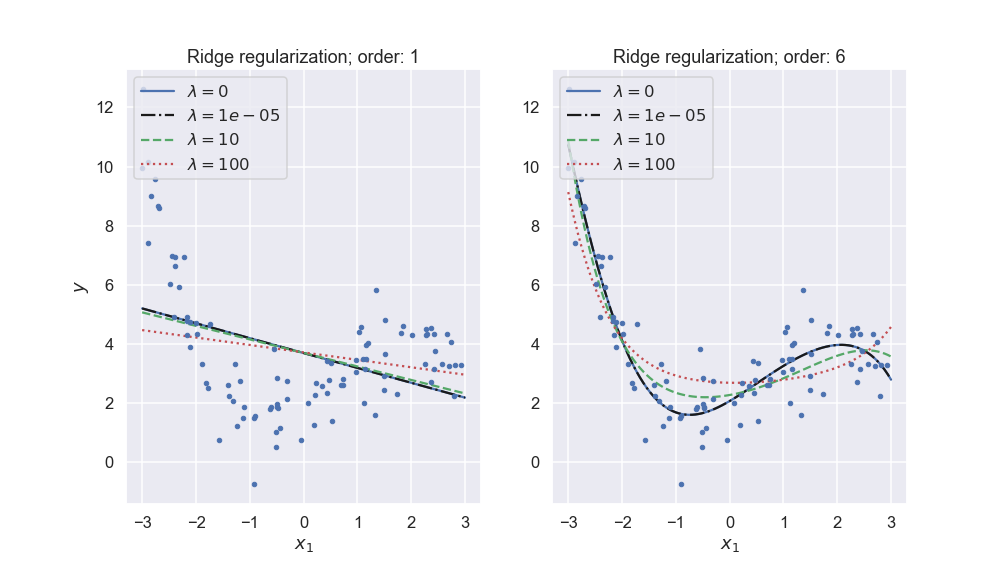
\includegraphics[width=0.9\linewidth]{fig/ridge_reg.png}}
  \caption{
  Ridge regularization with different penalty parameters $\lambda$ for different polynomial models of our noisy data set. \label{fig-ridge_reg}
  }
\end{figure}
%\clearpage % flush figures fig-ridge_reg




% !split
\subsection{More on Ridge Regression}

Using the matrix-vector expression for Ridge regression,

\[
C(\bm{X},\bm{\theta})=\frac{1}{n}\left\{(\bm{y}-\bm{X}\bm{\theta})^T(\bm{y}-\bm{X}\bm{\theta})\right\}+\lambda\bm{\theta}^T\bm{\theta},
\]

by taking the derivatives with respect to $\bm{\theta}$ we obtain then
a slightly modified matrix inversion problem which for finite values
of $\lambda$ does not suffer from singularity problems. We obtain

\[
\bm{\theta}^{\mathrm{Ridge}} = \left(\bm{X}^T\bm{X}+\lambda\bm{I}\right)^{-1}\bm{X}^T\bm{y},
\]

with $\bm{I}$ being a $p\times p$ identity matrix 

We see that Ridge regression is nothing but the standard
OLS with a modified diagonal term added to $\bm{X}^T\bm{X}$. The
consequences, in particular for our discussion of the bias-variance
are rather interesting. Ridge regression imposes a constraint on the model parameters
\[
\sum_{i=0}^{p-1} \theta_i^2 \leq t,
\]
with $t$ a finite positive number. 

For more discussions of Ridge and Lasso regression, see: \href{{https://arxiv.org/abs/1509.09169}}{Wessel van Wieringen's} article or \href{{https://arxiv.org/abs/1803.08823}}{Mehta et al's article}.

% !split
\subsection{The bias-variance tradeoff}

We will discuss the bias-variance tradeoff in the context of
continuous predictions such as regression. However, many of the
intuitions and ideas discussed here also carry over to classification
tasks. Consider a dataset $\mathcal{L}$ consisting of the data
$\mathbf{X}_\mathcal{L}=\{(y_j, \boldsymbol{x}_j), j=0\ldots n-1\}$. 

Let us assume that the data with experimental noise is generated from a true model
\[
\bm{y}=f(\boldsymbol{x}) + \bm{\epsilon}_\mathrm{exp},
\]
where $\bm{\epsilon}_\mathrm{exp}$ is a vector of random variables. We will assume that these are independent and identically distributed (i.i.d), each one described by a normal (Gaussian) distribution with expectation (mean) value zero and variance $\sigma^2_\mathrm{exp}$.

In our derivation of the ordinary least squares method we defined then
an approximation to the function $f$ in terms of the parameters
$\bm{\theta}$ and the design matrix $\bm{X}$ which embody our model,
that is 
\[
\bm{f}(\bm{x}) \approx \bm{\tilde{f}}(\bm{\theta}) \equiv \bm{\tilde{y}}=\bm{X}\bm{\theta}. 
\]
The relation between the true description and our model is
\[
f_i = \tilde{y}_i + \bm{\epsilon}_{\mathrm{model},i}.
\]

Thereafter we found the optimum set of model parameters $\bm{\theta}$ by minimizing the mean-squared (model) error via the so-called cost function
\[
C(\bm{X},\bm{\theta}) =\frac{1}{n}\sum_{i=0}^{n-1}(y_i-\tilde{y}_i)^2 = 
\left[ \begin{array}{c}
\mathrm{assume}\\
\mathrm{i.i.d.~samples}
\end{array} \right]
\approx
\mathbb{E}\left[(y-\tilde{y})^2\right],
\]
where we have made the key assumption that the residuals $(\bm{y}-\bm{\tilde{y}})$ are independent and identically distributed (i.i.d.) random variables, i.e.~these are samples from a single underlying probability distribution. Remember that $\mathbb{E}(t)$ denotes the expectation value for the random variable $t$. In this context we also remind that the variance is given by $\mathrm{Var}(t) = \mathbb{E} \left[ \left(t -  \mathbb{E}(t)\right)^2 \right]$.

We can rewrite this expectation value as 
\[
\mathbb{E}\left[(y-\tilde{y})^2\right]=\frac{1}{n}\sum_i(f_i-\mathbb{E}\left[\tilde{y}\right])^2+\frac{1}{n}\sum_i(\tilde{y}_i-\mathbb{E}\left[\tilde{y}\right])^2+\sigma^2_\mathrm{exp}.
\]

The first of the three terms represents the square of the bias of the learning
method, which can be thought of as the error caused by the simplifying
assumptions built into the method. The second term represents the
variance of the chosen model and finally the last terms is the irreducible error $\epsilon_\mathrm{exp}$. We will view these terms from a slightly different angle once we familiarise ourselves with Bayesian methods.

To derive this equation, we need to recall that the variance of $y$ and $\epsilon_\mathrm{exp}$ are both equal to $\sigma^2_\mathrm{exp}$. The mean value of $\epsilon_\mathrm{exp}$ is by definition equal to zero. Furthermore, the function $f$ is not a stochastic variable, idem for $\tilde{y}$.
We use a more compact notation in terms of the expectation value 
\[
\mathbb{E}\left[(y-\tilde{y})^2\right]=\mathbb{E}\left[({f}+\epsilon_\mathrm{exp}-\tilde{y})^2\right],
\]
and adding and subtracting $\mathbb{E}\left[\tilde{y}\right]$ we get
\[
\mathbb{E}\left[(y-\tilde{y})^2\right]=\mathbb{E}\left[({f}+\epsilon_\mathrm{exp}-\tilde{y}+\mathbb{E}\left[\tilde{y}\right]-\mathbb{E}\left[\tilde{y}\right])^2\right].
\]
We can rewrite this expression as a sum of three terms:
\begin{itemize}
\item The first one is the (squared) bias of the model plus the irreducible data error $\sigma_\mathrm{exp}^2$
\end{itemize}

\noindent
\[
\mathbb{E}\left[({f}+\epsilon_\mathrm{exp}-\mathbb{E}\left[\tilde{y}\right])^2\right] = \mathbb{E}\left[({f}-\mathbb{E}\left[\tilde{y}\right])^2\right] + \mathbb{E}\left[\epsilon_\mathrm{exp}^2\right]+0.
\]
\begin{itemize}
\item The second one is the variance of the model $\mathrm{Var}\left[ \tilde{y} \right]$
\end{itemize}

\noindent
\[
\mathbb{E}\left[(\mathbb{E}\left[\tilde{y}\right] - \tilde{y})^2\right],
\]
\begin{itemize}
\item and the last one is zero
\end{itemize}

\noindent
\[
2\mathbb{E}\left[(y-\mathbb{E}\left[\tilde{y}\right])(\mathbb{E}\left[\tilde{y}\right]-\tilde{y})\right] = 2\mathbb{E}\left[y-\mathbb{E}\left[\tilde{y}\right]\right] \left( \mathbb{E}\left[\mathbb{E}\left[\tilde{y}\right]\right] - \mathbb{E}\left[\tilde{y}\right]\right) = 0.
\]

The tradeoff between bias and variance is illustrated in Fig.~\ref{fig-bias_variance} from the demonstration notebook.


\begin{figure}[!ht]  % fig-bias_variance
  \centerline{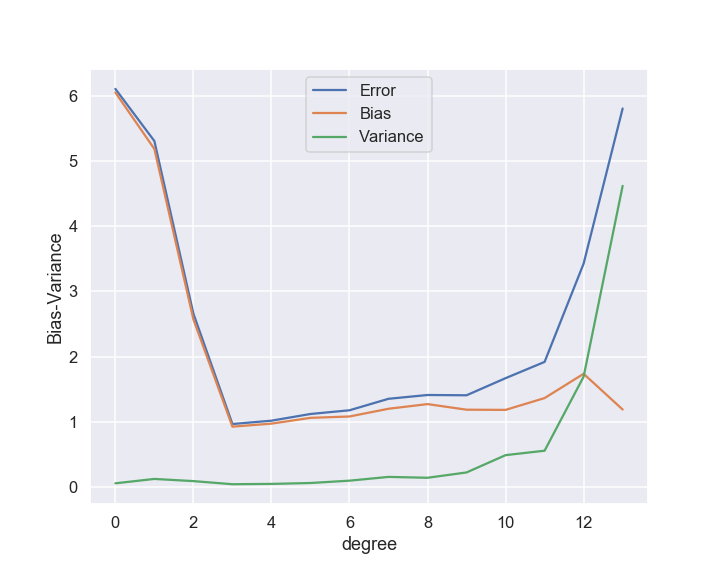
\includegraphics[width=0.8\linewidth]{fig/bias_variance.png}}
  \caption{
  The bias-variance for different polynomial models of our noisy data set. \label{fig-bias_variance}
  }
\end{figure}
%\clearpage % flush figures fig-bias_variance



% !split 
\subsection{Summing up}


The bias-variance tradeoff summarizes the fundamental tension in
machine learning, particularly supervised learning, between the
complexity of a model and the amount of training data needed to train
it.  Since data is often limited, in practice it is often useful to
use a less-complex model with higher bias, that is  a model whose asymptotic
performance is worse than another model because it is easier to
train and less sensitive to sampling noise arising from having a
finite-sized training dataset (smaller variance). 



The above equations tell us that in
order to minimize the expected validation error, we need to select a
statistical learning method that simultaneously achieves low variance
and low bias. Note that variance is inherently a nonnegative quantity,
and squared bias is also nonnegative. Hence, we see that the expected
validation MSE can never lie below $\mathrm{Var}(\bm{\epsilon}_\mathrm{exp}) \equiv \sigma^2_\mathrm{exp}$, the irreducible error.


What do we mean by the variance and bias of a statistical learning
method? The variance refers to the amount by which our model would change if we
estimated it using a different training data set. Since the training
data are used to fit the statistical learning method, different
training data sets  will result in a different estimate. But ideally the
estimate for our model should not vary too much between training
sets. However, if a method has high variance  then small changes in
the training data can result in large changes in the model. In general, more
flexible statistical methods have higher variance.


% !split 
\subsection{Model validation strategy}

Let us summarize the basic recipe for applying a supervise machine-learning model:

\begin{enumerate}
 \item Choose a class of models

 \item Choose model hyperparameters

 \item Fit the model to the training data

 \item Use the model for predictions
\end{enumerate}

\noindent
In our examples so far, the class of models has been linear regression models with polynomial basis functions. Hyperparameters then correspond to the choice of polynomial degree, and the Ridge regularization factor $\lambda$ if we use this technique, etc. 

In order to make an informed choice for these hyperparameters we need to validate that our model and its hyperparameters provide a good fit to the data. This important step is typically known as \emph{model validation}, and it most often involves splitting the data into two sets: the training set and the validation set. 

The model is then trained on the first set of data, while it is validated (by computing your choice of performance score) on the validation set.


\begin{question_mdfboxadmon}[Question]
Why is it important not to train and evaluate the model on the same data?
\end{question_mdfboxadmon} % title: Question




% !split 
\subsection{Cross-validation}

Cross-validation is a strategy to find model hyperparameters that yield a model with good prediction
performance. A common practice is to hold back some subset of the data from the training of the model and then use this holdout set to check the model performance. The splitting of data can be performed using the the \Verb!train_test_split! utility in Scikit-Learn.

One of these two data sets, called the 
\emph{training set}, plays the role of \textbf{original} data on which the model is
built. The second of these data sets, called the \emph{validation set}, plays the
role of the \textbf{novel} data and is used to evaluate the prediction
performance (often operationalized as the log-likelihood or the
prediction error: MSE or R2 score) of the model built on the training data set. This
procedure (model building and prediction evaluation on training and
validation set, respectively) is done for a collection of possible choices for the hyperparameters. The parameter that yields the model with
the best prediction performance is to be preferred. 

% !split
The validation set approach is conceptually simple and is easy to implement. But it has two potential drawbacks:

\begin{itemize}
\item The validation estimate of the validation error rate can be highly variable, depending on precisely which observations are included in the training set and which observations are included in the validation set. There might be data points that are critical for training the model, and the performance metric will be very bad if those happen to be excluded from the training set.

\item In the validation approach, only a subset of the observations, those that are included in the training set rather than in the validation set are used to fit the model. Since statistical methods tend to perform worse when trained on fewer observations, this suggests that the validation set error rate may tend to overestimate the validation error rate for the model fit on the entire data set.
\end{itemize}

\noindent
% !split 
To reduce the sensitivity on a particular data split, one can use perform several different splits. For each split the model is fit using the training data and
evaluated on the corresponding validation set. The hyperparameter that performs best on average (in some sense) is then selected.


% !split 
\paragraph{$k$-fold cross validation cross-validation.}
When the repetitive splitting of the data set is done randomly,
samples may accidently end up in a fast majority of the splits in
either training or validation set. Such samples may have an unbalanced
influence on either model building or prediction evaluation. To avoid
this $k$-fold cross-validation is an approach to structure the data splitting. The
samples are divided into $k$ more or less equally sized, exhaustive and
mutually exclusive subsets. In turn (at each split) one of these
subsets plays the role of the validation set while the union of the
remaining subsets constitutes the training set. Such a splitting
warrants a balanced representation of each sample in both training and
validation set over the splits. Still the division into the $k$ subsets
involves a degree of randomness. This may be fully excluded when
choosing $k=n$. This particular case is referred to as leave-one-out
cross-validation (LOOCV). 

% !split 
\paragraph{How to set up cross-validation.}
\begin{itemize}
\item Define a range of interest for the  model hyperparameter(s) $\lambda$.

\item Divide the data set $\mathcal{D} = \{1, \ldots, n\}$ into $k$ exhaustive and mutually exclusive subsets $\mathcal{D}_{i} \subset \mathcal{D}$ for $i=1,\ldots,k$, and $\mathcal{D}_{i} \cap \mathcal{D}_{j} = \emptyset$ for $i \neq j$.

\item For $i \in \{1, \ldots, k\}$:
\begin{itemize}

  \item Define $\mathcal{D}_{i}$ as the validation set and $\mathcal{D}_{-i} = \mathcal{D} - \mathcal{D}_i$ as the training set.

  \item Fit the model for each choice of the hyperparameter using the training set, which will give a best fit $\bm{\theta}_{-i}(\lambda)$.

  \item Evaluate the prediction performance of these models on the validation set by the MAE, MSE, or the R2 score function. 

\end{itemize}

\noindent
\item Average the prediction performances of the validation sets at each grid point of the hyperparameter by computing the \emph{cross-validated error}. It is an estimate of the prediction performance of the model corresponding to this value of the penalty parameter on novel data. For example, using the MSE measure it is defined as
\end{itemize}

\noindent
\begin{align*}
\mathrm{CV}_k(\lambda) \equiv
\frac{1}{k} \sum_{i = 1}^k \mathrm{MSE} \left( \bm{\theta}_{-i}(\lambda) \right).
\end{align*}

\begin{itemize}
\item The value of the hyperparameter that minimizes the cross-validated error is the value of choice. 
\end{itemize}

\noindent
\[
\lambda^* = \underset{\lambda}{\operatorname{argmin}}
\mathrm{CV}_k(\lambda)
\].



% !split
\section{Gradient-descent optimization}

With the linear regression model we could find the best fit parameters by solving the normal equation. Although we could encounter problems associated with inverting a matrix, we do in principle have a closed-form expression for the model parameters.

In general, the problem of optimizing the model parameters is a very difficult one. We will return to the optimization problem later in this course, but will just briefly introduce the most common class of optimization algorithms: \emph{Gradient descent} methods. The general idea of Gradient descent is to tweak parameters iteratively in order to minimize a cost function.

Let us start with a cost function for our model such as the chi-squared function that was introduced in the Linear Regression lecture:

\[
\chi^2(\bm{\theta})=\frac{1}{n}\sum_{i=0}^{n-1}\frac{\left(y_i-\tilde{y}_i\right)^2}{\sigma_i^2}=\frac{1}{n}\left\{\left(\bm{y}-\bm{\tilde{y}}\right)^T \bm{\Sigma}^{-1}\left(\bm{y}-\bm{\tilde{y}}\right)\right\},
\]

Instead of finding a matrix equation for the vector $\bm{\theta}$ that minimizes this measure we will describe an iterative procedure:

\begin{itemize}
\item Make a \emph{random initialization} of the parameter vector $\bm{\theta}_0$.

\item Compute the gradient of the cost function with respect to the parameters (note that this can be done analytically for the linear regression model). Let us denote this gradient vector $\bm{\nabla}_{\bm{\theta}} \left( \chi^2 \right)$.

\item Once you have the gradient vector, which points uphill, just go in the opposite direction to go downhill. This means subtracting $\eta \bm{\nabla}_{\bm{\theta}} \left( \chi^2 \right)$ from $\bm{\theta}_0$. Note that the magnitude of the step, $\eta$ is known as the learning rate and becomes another hyperparameter that needs to be tuned.

\item Continue this process iteratively until the gradient vector $\bm{\nabla}_{\bm{\theta}} \left( \chi^2 \right)$ is close to zero.
\end{itemize}

\noindent
Gradient descent is a general optimization algorithm. However, there are several important issues that should be known before using it:

\begin{enumerate}
\item It requires the computation of partial derivatives of the cost function. This is straight-forward for the linear regression method, but can be difficult for other models. The use of \emph{automatic differentiation} is very popular in the ML community,and is well worth exploring. 

\item In principle, gradient descent works well for convex cost functions, i.e.~where the gradient will eventually direct you to the position of the global minimum. Again, the linear regression problem is favorable because you can show that the cost function has that property. However, most cost functions---in particular in many dimensions---correspond to very \emph{complicated surfaces with many local minima}. In those cases, gradient descent is often not a good method.
\end{enumerate}

\noindent
There are variations of gradient descent that uses only fractions of the training set for computation of the gradient. In particular, stochastic gradient descent and mini-batch gradient descent.

% !split
\subsection{Learning curves}

The performance of your model will depend on the amount of data that is used for training. When using iterative optimization approaches, such as gradient descent, it will also depend on the number of training iterations. In order to monitor this dependence one usually plots \emph{learning curves}.

Learning curves are plots of the model's performance on both the training and the validation sets, measured by some performance metric such as the mean squared error. This measure is plotted as a function of the size of the training set, or alternatively as a function of the training iterations.


\begin{figure}[!ht]  % fig-learning_curve
  \centerline{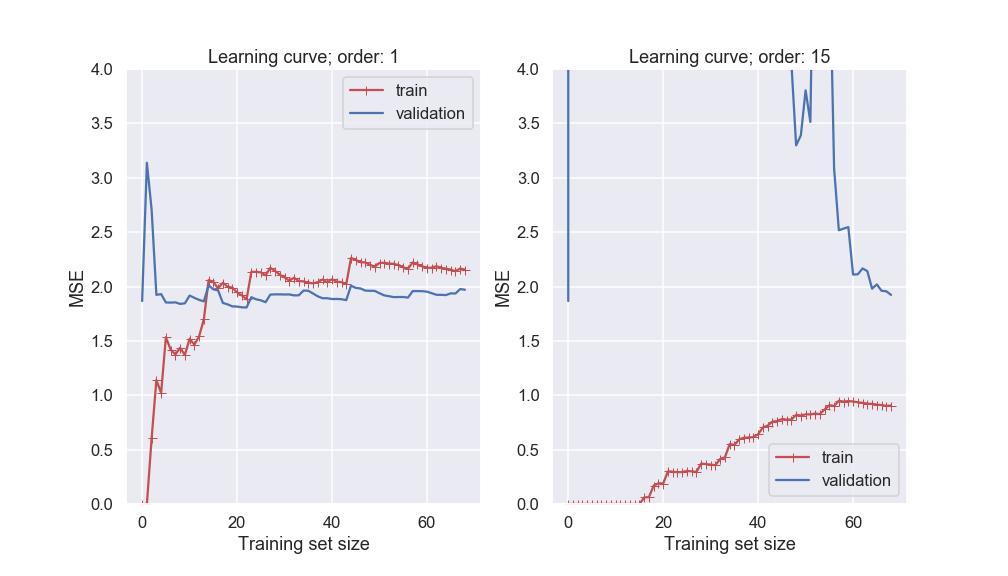
\includegraphics[width=0.8\linewidth]{fig/learning_curve.png}}
  \caption{
  Learning curves for different polynomial models of our noisy data set as a function of the size of the training data set. \label{fig-learning_curve}
  }
\end{figure}
%\clearpage % flush figures fig-learning_curve


Several features in the left-hand panel deserves to be mentioned:

\begin{enumerate}
\item The performance on the training set starts at zero when only 1-2 data are in the training set.

\item The error on the training set then increases steadily as more data is added. 

\item It finally reaches a plateau.

\item The validation error is initially very high, but reaches a plateau that is very close to the training error.
\end{enumerate}

\noindent
The learning curves in the right hand panel are similar to the underfitting model; but there are some important differences:

\begin{enumerate}
\item The training error is much smaller than with the linear model.

\item There is no clear plateau.

\item There is a gap between the curves, which implies that the model performs significantly better on the training data than on the validation set.
\end{enumerate}

\noindent
Both these examples that we have just studied demonstrate again the so called \emph{bias-variance tradeoff}.

\begin{itemize}
 \item A high bias model has a relatively large error, most probably due to wrong assumptions about the data features.

 \item A high variance model is excessively sensitive to small variations in the training data.

 \item The irreducible error is due to the noisiness of the data itself. It can only be reduced by obtaining better data.
\end{itemize}

\noindent
We seek a more systematic way of distinguishing between under- and overfitting models, and for quantification of the different kinds of errors. We will find that \textbf{Bayesian statistics} has the promise to deliver on that ultimate goal.


% ------------------- end of main content ---------------

% #ifdef PREAMBLE
\end{document}
% #endif

